\section{Desenvolvimento}
\label{sec:desenvolvimento}
    \subsection{Circuito}
    \label{sec:circuito}
        \indent O circuito proposto é mostrado na Figura \ref{fig:figure}.
        Como parâmetros iniciais, determinou-se os valores abaixo.\\

        \indent Parâmetros iniciais
        \begin{itemize}
            \item $V_{cc} = 12V$
            \item $R_1 = 10K\Omega$
            \item $R_2 = 3.9K\Omega$
            \item $R_3 = 2.2K\Omega$
            \item $R_4 = 820\Omega$
            \item $C_1 = 10\mu F$
            \item $C_2 = 50\mu F$
        \end{itemize}
        \onehalfspace

        \indent Os parâmetros obtidos foram:
        \begin{itemize}
            \item $I_c = 5 mA$
            \item $V_{ce} = 10V$
            \item $V_{re} = 0.10\cdot V_{cc}$
            \item $V_{cc} = 15\cdot V$
        \end{itemize}

    \indent Ao procurar informações sobre o transistor BC-547, foi possível determinar que trata-se de um transistor NPN de baixa potência, com uma corrente de saturação de $1,8 \cdot 10^{-14} A$ e uma tensão de saturação de $45 V$, mantendo uma faixa de ganho entre $110 hFE$ e $800 hFE$\\

    \indent O transistor BC-547 possui o seguinte diagrama para a polarização de coletor e emissor:
    \begin{figure}[h!]
        \centering
        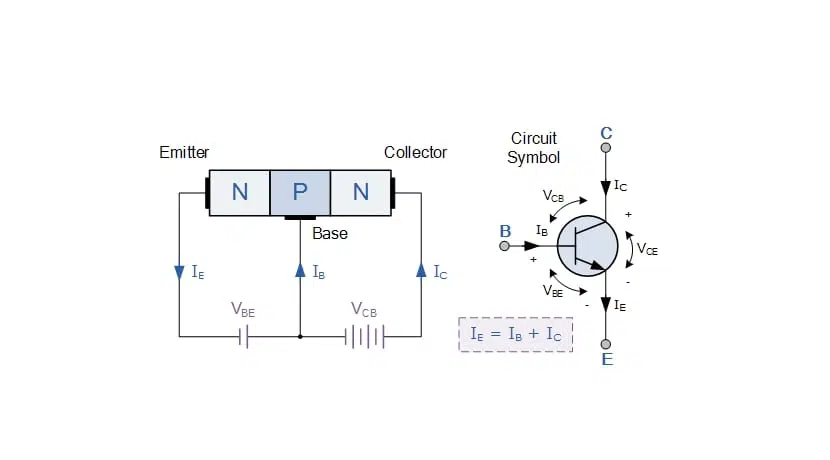
\includegraphics[width=1\textwidth]{pictures/img.png}
        \caption{Diagrama de polarização do transistor BC-547}
        \label{fig:BC547}
    \end{figure}


    \subsection{Procedimentos}
    \label{subsec:procedimentos}
    \indent Para a realização dos testes, foi utilizado um osciloscópio, um multímetro digital e um gerador de sinais.
    O circuito foi montado em uma protoboard com terminais para fonte assimétrica, e os valores de resistores e capacitores foram ajustados para que o circuito funcionasse corretamente.\\

    \indent O circuito foi ligado à fonte de 18V, e o osciloscópio foi conectado ao pino de saída do circuito.
    O gerador de sinais foi conectado ao pino de entrada do circuito, e o multímetro foi conectado ao pino de saída do circuito, sendo configurado para gerar uma onda quadrada com frequência de 1kHz, e o osciloscópio foi configurado para mostrar a onda de saída do circuito.
    O multímetro foi configurado para medir a tensão no pino de saída do circuito, e o osciloscópio foi configurado para mostrar a onda de saída do circuito.\\

    \begin{figure}[h!]
        \centering
        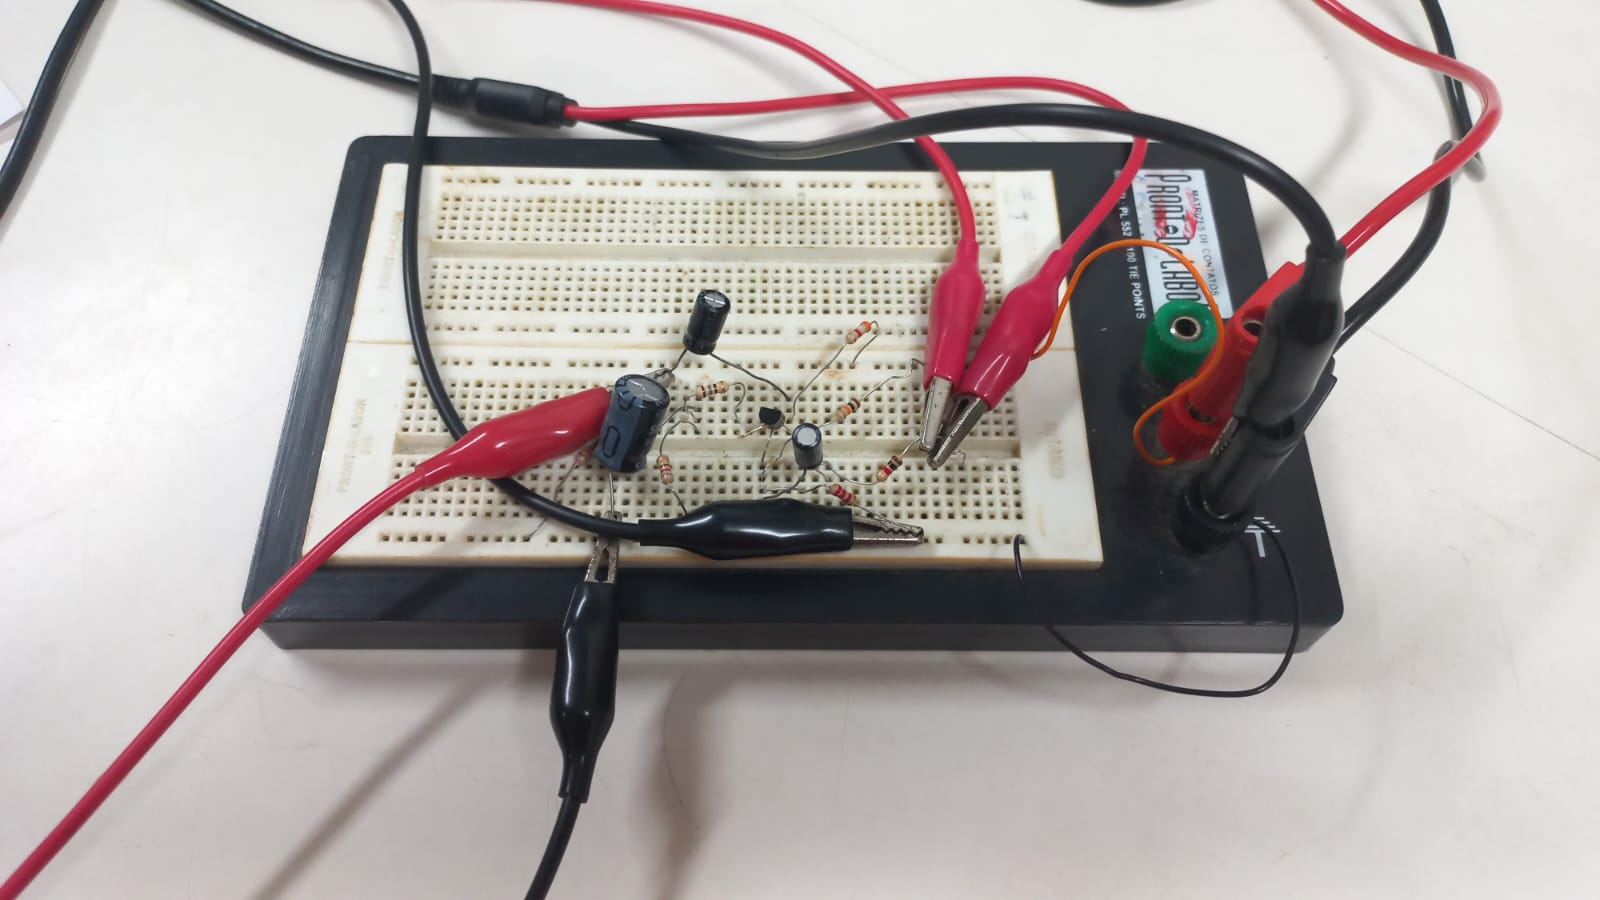
\includegraphics[width=1\textwidth]{pictures/circuito_montado.jpeg}
        \caption{Circuito montado pra testes na protoboard}
        \label{fig:fig1}
    \end{figure}

    \indent No primeiro teste, foi utilizado o gerador de sinais para gerar uma onda quadrada com frequência de 1kHz, e o osciloscópio foi configurado para mostrar a onda de saída do circuito.
     As imputs e outputs do circuito foram, respectivamente $V_{entrada} = 200mV$, $V_{saida} = 1V$, isso para uma alimentação de $10V$ no circuito, essas informações são mostradas na figura a seguir:
    \begin{figure}[h!]
        \centering
        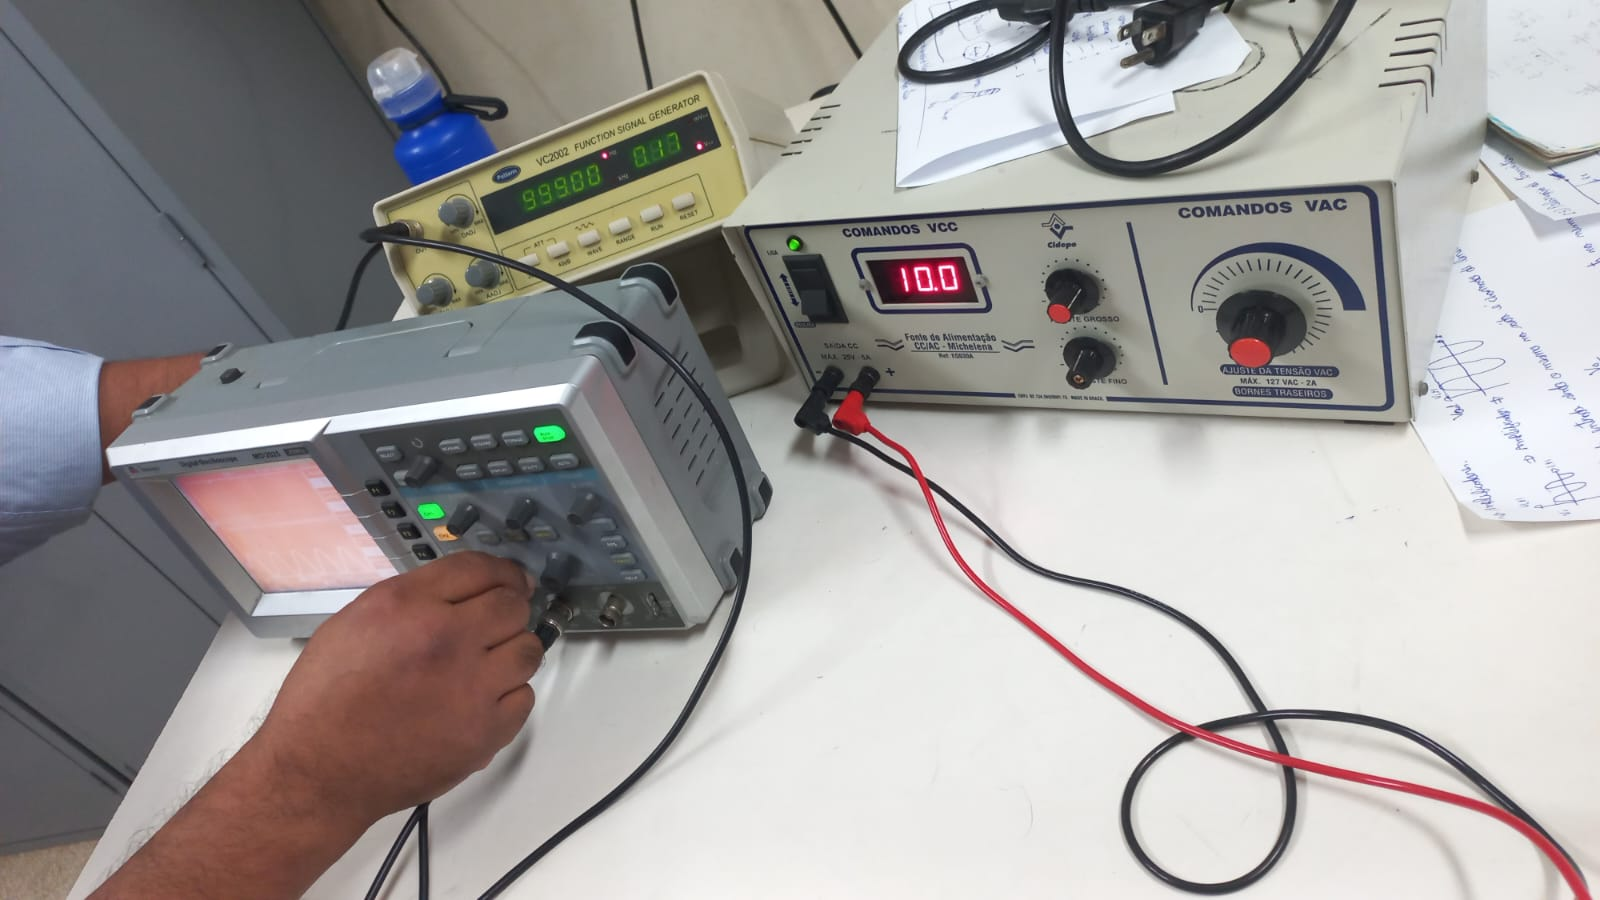
\includegraphics[width=0.4\textwidth]{pictures/bancada de analise.jpeg} \quad
        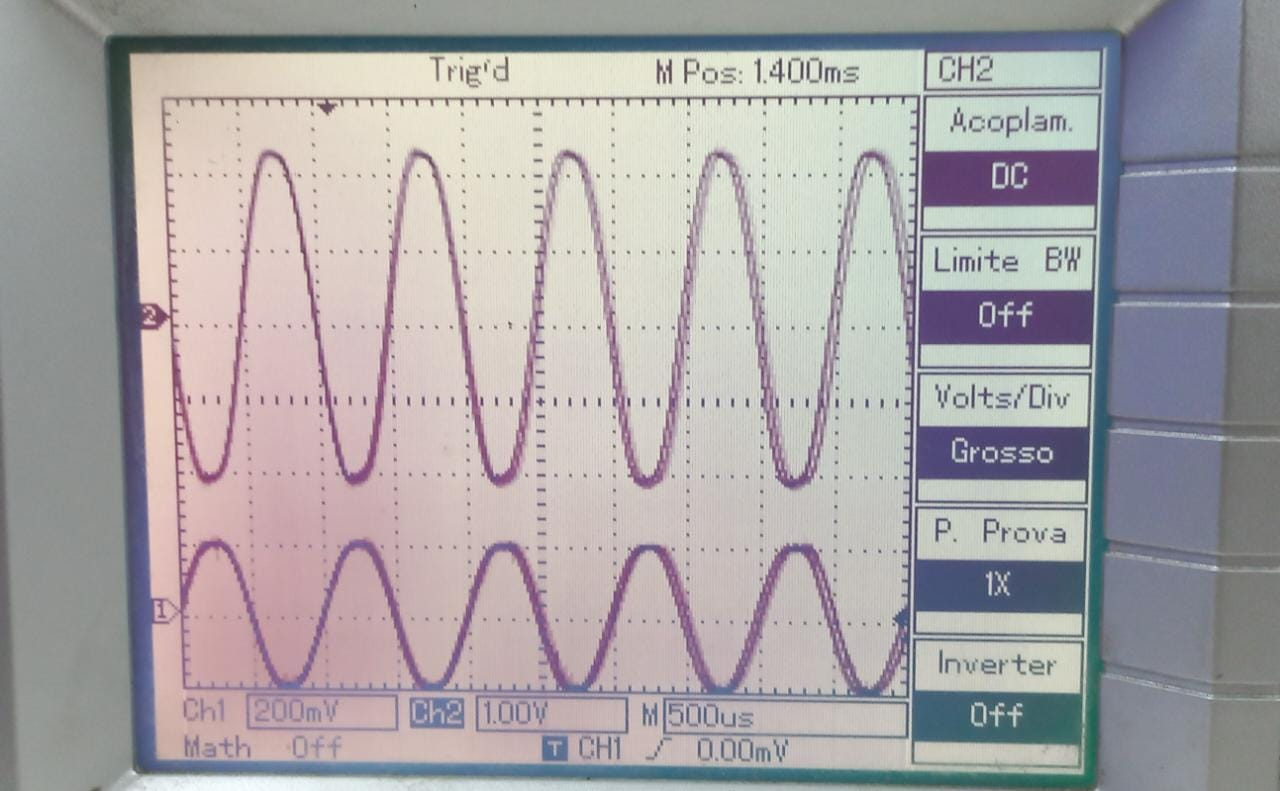
\includegraphics[width=0.4\textwidth]{pictures/osciloscopio teste 1.jpeg}
        \caption{Primeiros Testes de bancada}
        \label{fig:fig2e4}
    \end{figure}

    \indent O ganho observado foi de 5 vezes a entrada, e para o teste em específico, a tensão de saída foi de $1V$.

    \newpage

    \indent No segundo teste, a entrada e saída foram alteradas para $V_{entrada} = 1.14V$ e $V_{saida} = 5.2V$, respectivamente, e o ganho observado foi de 4.56, e para o teste em específico, a tensão em que o sistema foi ligado foi de $18V$.

    \begin{figure}[h!]
        \centering
        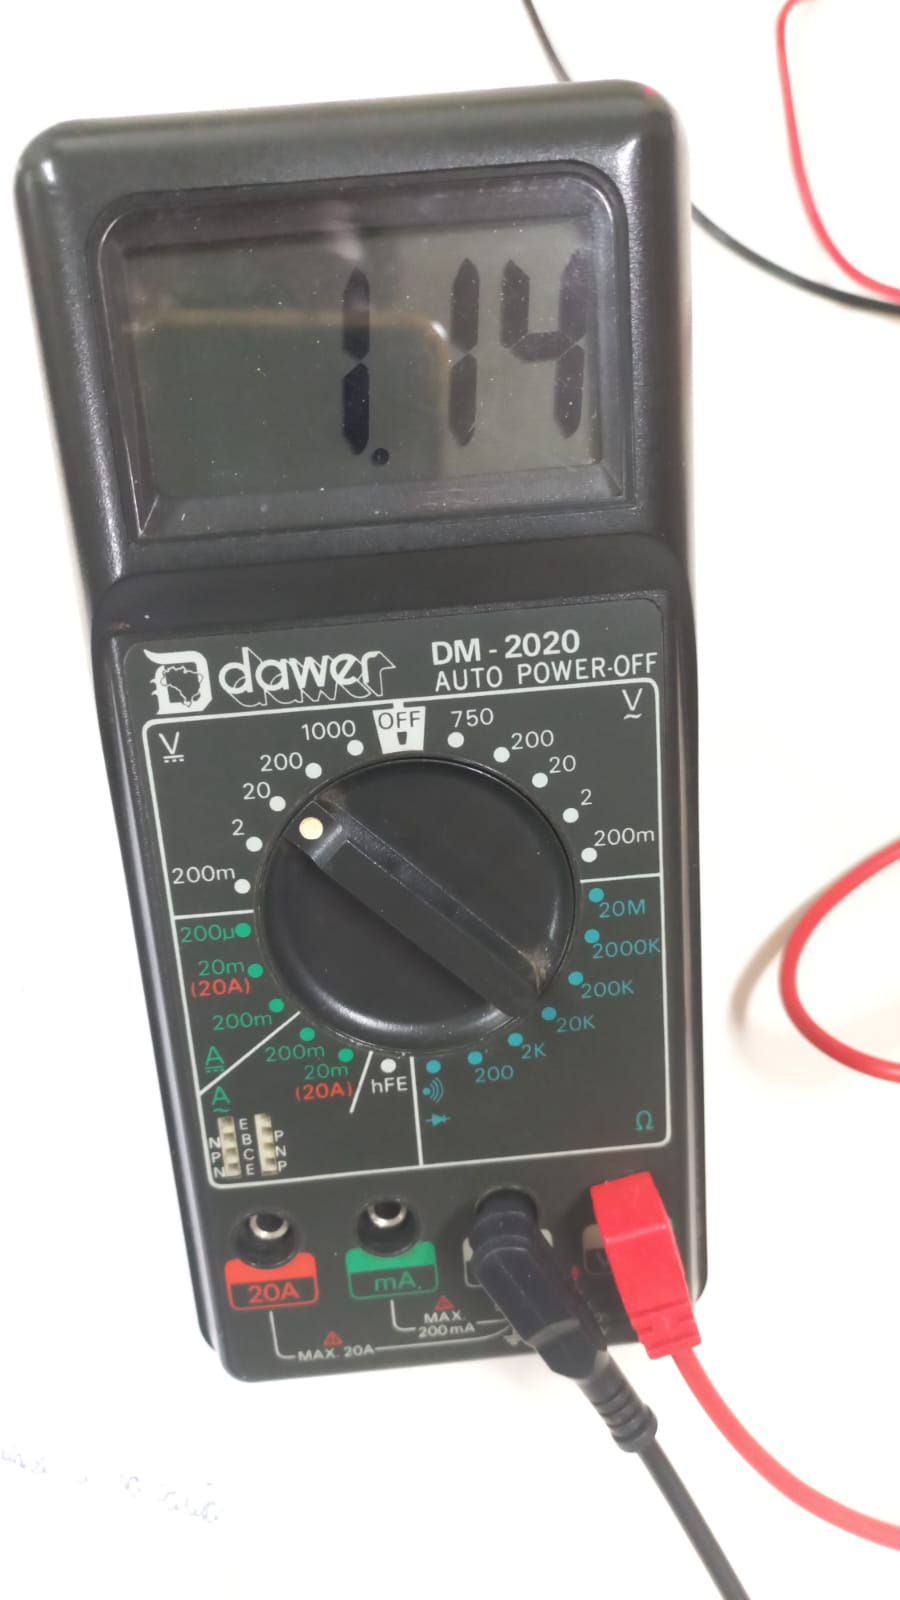
\includegraphics[width=0.4\textwidth]{pictures/mult114.jpeg} \quad
        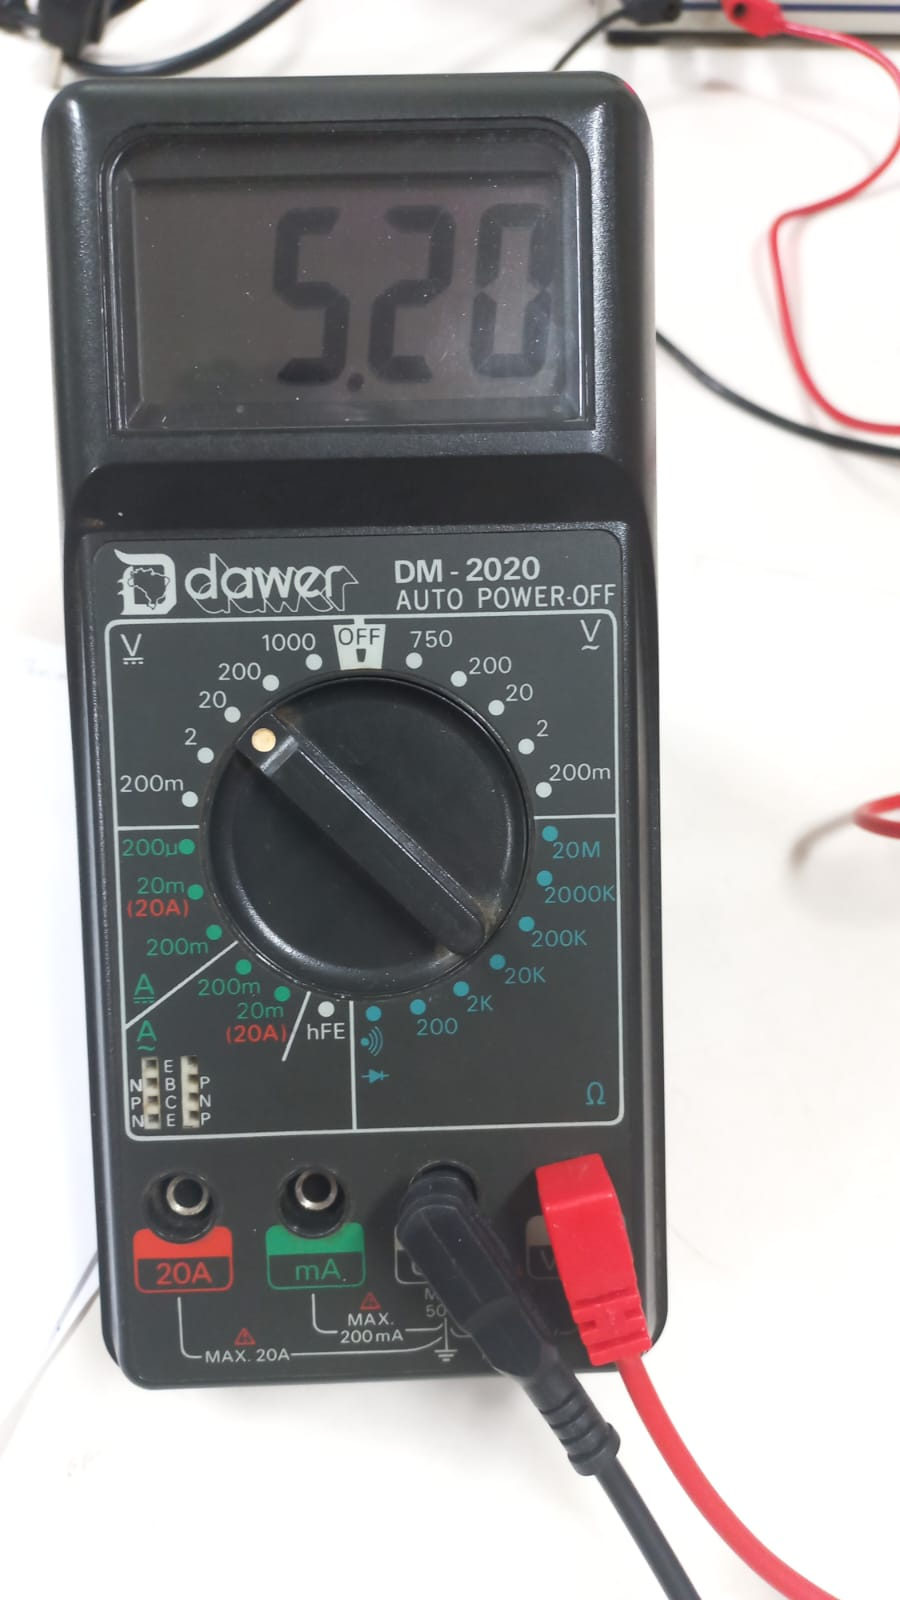
\includegraphics[width=0.4\textwidth]{pictures/mult52.jpeg}
        \caption{Segundos Testes de bancada}
        \label{fig:fig5e6}
    \end{figure}

